\section{Issue \#2508}\label{issue-2508}

\subsection{The issue}\label{the-issue}

The first issue we intend to tackle consists in a feature which allows
the user to disable quotes/parentheses/brackets automatic matching. This
issue is being tracked in GitHub, and it's the issue \#2508.

\subsection{Requirements}\label{requirements}

Boostnote is coded mainly in javascript, so, even though it's a Desktop
application it has a web - like development.

Some users expressed that they do not like this feature in a context
other than coding, as such solving this issue will allow the user to
disable the automatic matching function when desired.

\begin{figure}
\centering
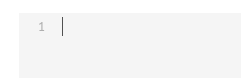
\includegraphics[height=0.93750in]{../noBracketsEx.png}
\caption{No Brackets}
\end{figure}

\begin{figure}
\centering
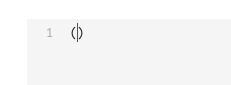
\includegraphics[height=1.04167in]{../bracketsEx.png}
\caption{With Brackets}
\end{figure}

In the pictures above, between both of them, just the first parenthesis
were inserted by the user. The other was automatically inserted and the
cursor stays inside of them.

It was also requested that, when the option to automatically match
parentheses is enabled, that the user should be able to choose which
characters he desires to have paired/tripled/exploded.

\subsection{Source Code Files}\label{source-code-files}

To add new options to the preference tab, the file
\emph{browser/main/modals/PreferencesModal/UiTab.js} will need to
change.

The file \emph{browser/main/lib/ConfigManager.js} contains default
values for the configuration, therefore some new fields will need to be
added.

The following files represent several types of editors, which will
suffer changes to accomudate the new configuration options:

\begin{itemize}
\tightlist
\item
  \emph{browser/main/modals/PreferencesModal/SnippetTab.js}
\item
  \emph{browser/main/modals/PreferencesModal/SnippetEditor.js}
\item
  \emph{browser/main/Detail/SnippetNoteDetail.js}
\item
  \emph{browser/components/MarkdownSplitEditor.js}
\item
  \emph{browser/components/MarkdownSplitEditor.js}
\item
  \emph{browser/components/MarkdownSplitEditor.js}
\end{itemize}

\subsection{Relevant System
Architecture}\label{relevant-system-architecture}

Before tackling the issues, a look needs to be taken over the overall
architecture of the program. For brevity, the following diagrams have
been simplified to show only the relevant architecture.

In the following diagram the main components of the board are
represented:

\begin{itemize}
\item
  Local Storage: Stores permanent files containing the programs
  information, i.e.~configuration.
\item
  Configuration Manager: Retrieves the current configuration from memory
  and saves any changes made to it.
\item
  Update Server: Checks the remote repository for any updates to the
  program.
\item
  Markdown Renderer: External library to convert markdown to html.
\item
  CodeMirror: External library that textual input.
\end{itemize}

\begin{figure}
\centering
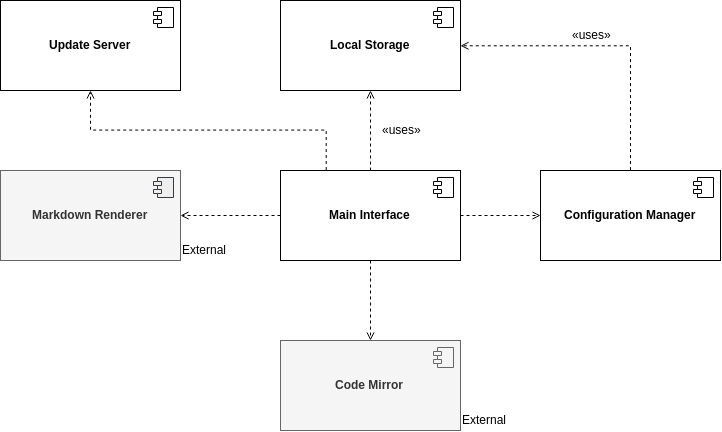
\includegraphics[height=3.12500in]{../ComponentDiagram.png}
\caption{Component Diagram}
\end{figure}

\begin{figure}
\centering

\includegraphics[height=4.16667in]{../ClassDiagram.png}
\caption{Class Diagram}
\end{figure}

Following the components, it can be seen a simplified version of the
class diagram, in which some of the classes implemented in the project
can be seen, including those that need to be modified.

Finally, it is relevant to show how the program loads changes made to
the configuration.

\begin{figure}
\centering
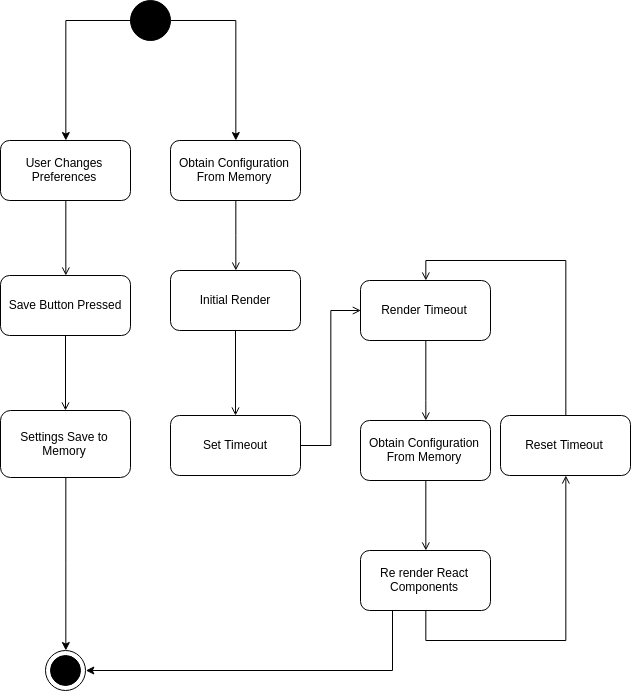
\includegraphics[height=4.16667in]{../activityDiagram.png}
\caption{Activity Diagram}
\end{figure}

\subsection{Design of the fix}\label{design-of-the-fix}

As it is shown in the component diagram, the program uses a JavaScript
package called CodeMirror to handle the main textual input. This package
can be configured to automatically close brakets, by passing a string
containing which characters are to be closed with which characeters. In
fact, CodeMirror can have 3 types of auto bracket matching:

\begin{itemize}
\item
  Matching pairs - When a given character is typed, it's closing
  character is added right after.
\item
  Matching triplets - When 3 character of given type are inserted in
  sequence, this same characters are repeated right after, i.e.
  \texttt{\textquotesingle{}\textquotesingle{}\textquotesingle{}}
  becomes
  \texttt{\textquotesingle{}\textquotesingle{}\textquotesingle{}\textquotesingle{}\textquotesingle{}\textquotesingle{}}.
\item
  Exploding pair - When a new line is inserted between one of these
  pairs, the second character moves 2 lines down.
\end{itemize}

To make use of this feature, 3 fields (one for each type) can be added
to the preferences, so that the value saved in these can be passed down
to the editor along with all other configurations. To change these
fields, 3 textboxes can be added to the interface tab in the preferences
window.

When the configuration is changed and a new render is needed, the React
framework only changes the components that suffered changes in its
attributes, therefore the function that verifies such updates must be
updated.

Finally, these new fiels must have default values, these can take the
strings that are being used to permanently configure o CodeMirror in the
current version of the program. 

\section{Issue \#1885}\label{issue-1885}

\subsection{The issue}\label{the-issue-1}

The second issue we intend to solve consists in an improvement which
highlights a folder when it's hovered when moving notes between folders.
This issue is being tracked in GitHub, and it's the issue \#1885.

\subsection{Requirements}\label{requirements-1}

Boostnote is coded mainly in javascript, so, even though it's a Desktop
application it has a web - like development.

It's not quite an issue, more of a request for an improvement to the
application. It was requested that when moving notes between folders
that the hovered folder was highlighted to help understand the folder
that was being selected as a destination for the note being picked.

\begin{figure}
\centering
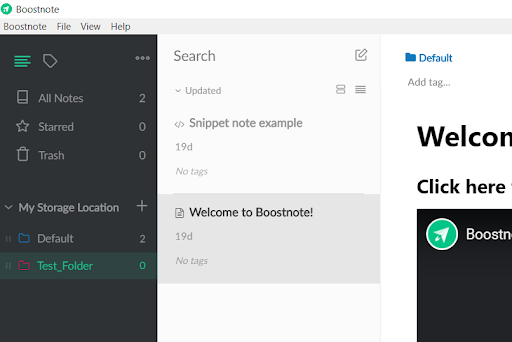
\includegraphics[height=2.08333in]{../hoveredWithMouseEx.png}
\caption{Mouse over folder}
\end{figure}

\begin{figure}
\centering
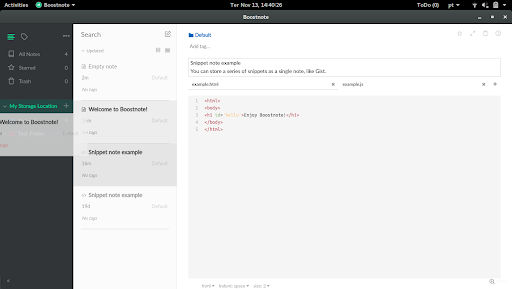
\includegraphics[height=2.08333in]{../hoveredWithNoteEx.png}
\caption{Dragged note over folder}
\end{figure}

In the top image we have the hovered folder being highlighted. The
objective of this issue is to produce the same effect when, while
dragging a note, the cursor hovers a folder. As we can see in the bottom
image no highlighting is done when hovering a folder while dragging a
note.

\section{Source Code Files}\label{source-code-files-1}

The file \emph{browser/main/SideNav/StorageItem.js} handles the
detection of the cursor when a note is dragged over and each of the
elements implemented in the previous file have their style in
\emph{browser/main/SideNav/StorageItem.styl}

\subsection{Relevant System
Architecture}\label{relevant-system-architecture-1}

Before tackling the issues, a look needs to be taken over the overall
architecture of the program. For brevity, the following diagrams have
been simplified to show only the relevant architecture.

In the following diagram the main components of the board are
represented:

\begin{itemize}
\item
  Local Storage: Stores permanent files containing the programs
  information, i.e.~configuration.
\item
  Configuration Manager: Retrieves the current configuration from memory
  and saves any changes made to it.
\item
  Update Server: Checks the remote repository for any updates to the
  program.
\item
  Markdown Renderer: External library to convert markdown to html.
\item
  CodeMirror: External library that textual input.
\end{itemize}

\begin{figure}
\centering
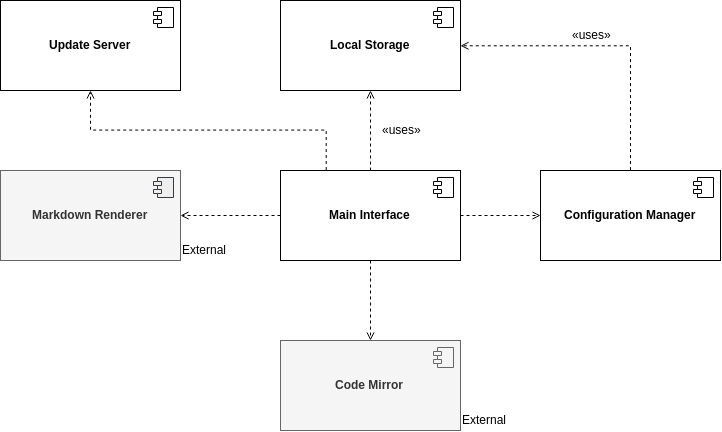
\includegraphics[height=3.12500in]{../ComponentDiagram.png}
\caption{Component Diagram}
\end{figure}

\begin{figure}
\centering

\includegraphics[height=4.16667in]{../ClassDiagram.png}
\caption{Class Diagram}
\end{figure}

Following the components, it can be seen a simplified version of the
class diagram, in which some of the classes implemented in the project
can be seen, including those that need to be modified.

For this issue is relevant to show the relevant states of the folders in
the side navigation bar.

\begin{figure}
\centering
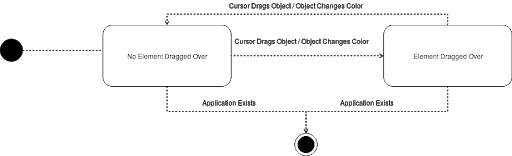
\includegraphics[width=6.25000in]{../stateDiagram.png}
\caption{State Diagram}
\end{figure}

\section{Design of the fix}\label{design-of-the-fix-1}

The fix for this problem is rather simple. The functionality of moving
notes between folders by dragging them already exists, so the hover of a
note over a folder is already handled. The only needed implementation
was to change the styling of the destination folder when it was hovered.
So the fix will consist in changing the background color of a folder
hovered with a note to be the same as the color of a folder when hovered
just with the mouse.
